\chapter{Data storage}
Data storage is important in a system like a windmill farm.
A lot of data must be persisted like weather data, health data of the different parts of every turbine and production data.
These records are important both for immediate use to view the current state of the system but also for review in the future for instance to predict weather trends or replace worn down parts of turbine before they break completely.

Currently data is aggregated from each turbine and stored on a central node.
This node will over time aggregate hundreds of gigabytes of information.
The data on the node is secured by backup but it is still a single point of failure.
Take out the data storage node or the communication to it and a lot of information will be lost.

By distributing the data of the system between all the connected nodes we achieve better redundancy because the data is present on many different nodes.
Should a node become unavailable another node can communicate the same data in effect strengthening the availability of the system.

This chapter contains a description of a number of relevant storage technologies and a discussion of which technology is the best suited for a system like the Siemens case.

\section{Relational storage, SQL}
The traditional way of storing data is in a Relational Database Management System(RDBMS).
These databases rely on a schema to arrange data in tables and their relations.
Using SQL it is easy to query data and to do aggregate operations.
RDBMSs support ACID transactions which ensures operations in the database are processed reliably.

A shortcoming of the RDBMSs is the problem with object-relational mapping also known as the Impedance Mismatch Problem\cite{Fowler:IntroNoSQL, Neward:TheVietnamOfComputerScience}.
The relational structure of the RDBMSs does not map well to the object-oriented structure the most popular programming languages encourage.
Often an object is an aggregate of a number of attributes.
In the context of the object-oriented program the object is seen as one entity.
In the context of the RDBMS the attributes of the object-oriented object is often scattered between multiple tables in the database to ensure consistency and avoid duplicate data.
This mismatch between object representation and relational representation can cause both performance problems, the JOIN operation in SQL is very costly, as well as considerable development time spent mapping one structure to the other.
The performance problem multiplies in a distributed database if the RDBMS must do JOIN operations across the network in order to aggregate data.

Another problem with a traditional RDBMS is that they are designed for vertical scaling\cite{Atzeni:TheRelationalModelIsDead}. If a traditional RDBMS has problems handling data the solution is to add a bigger harddrive or invest in a faster CPU. This makes sense in a world were hardware is very expensive like it was when the traditional RDBMSs saw the light of day\cite{Stonebraker:TheEndOfAnArchitecturalEra}. Today horizontal scaling is preferred. If a system has a problem with the data load add another machine or add five others if that is what it takes.

\section{Schema-less storage, NoSQL}
Since 2009 the schema-less storage methods have become increasingly popular.
Relational databases could no longer keep up with the task of storing and querying big data.
A new breed of schema-less storage systems became popular because they could handle some of the problems big data caused for the relational storage systems.
This new breed of databases are designed for horizontal scalability and without strict schemas allowing a more flexible data model. 
They are capable of handling huge amounts of data both for storage but also for analysis or batch operations.
The downside however is the lack of the ACID properties which results in a lower consistency and the lack of transactions. %TODO: Dårligt formuleret omskriv!

The schema-less databases can be divided roughly into four categories\cite{Fowler:IntroNoSQL, Moniruzzaman:NoSQLDatabaseNewEraOfDatabasesForBigDataAnalysis}, which will be described separately in the following sections.

\subsection{Document databases}
The document databases are designed to contain documents.
The documents contains attribute name/value pairs.
Attributes may vary between rows.
To retrieve data it is possible to search both on the attribute and the value.

Primary use include storing actual documents like emails and blog posts, or storage of semi-structured and aggregate data.

\begin{figure}
	\centering
	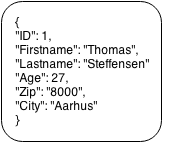
\includegraphics[scale=0.8]{Document.png} 
	\captionsetup{format=plain,font=footnotesize,labelfont={bf,defaultCapFont},labelsep=quad,singlelinecheck=no}
	\caption[Document store]{
		\label{fig:DocumentStore}
		\footnotesize{%
			Document store structure.
		} 
	}
\end{figure}

\subsection{Key-value stores}
The key-value stores can be compared to a hashmap since every entry has a key and an associated value. 
To retrieve data you search for the key. 
The values can contain any kind of data from simple text to lists or documents.

Primary use includes fast lookup for instance for user sessions or product lists.

\begin{figure}
	\centering
	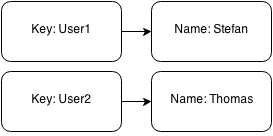
\includegraphics[scale=0.8]{KeyValue.png} 
	\captionsetup{format=plain,font=footnotesize,labelfont={bf,defaultCapFont},labelsep=quad,singlelinecheck=no}
	\caption[Key-value store]{
		\label{fig:KeyValueStore}
		\footnotesize{%
			Key-value store structure.
		} 
	}
\end{figure}

\subsection{Column-family stores}
Column-family stores keep related data stored together.
A column-family object consists of a key-value pair where the value contains columns of related data.

Primary use includes distributed data storage, batch processing of data and analytical processing for statistical use.

\begin{figure}
	\centering
	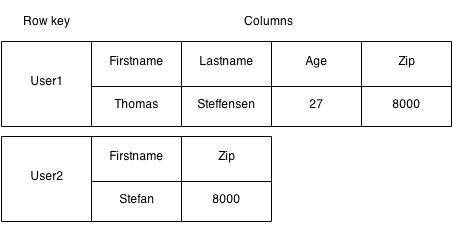
\includegraphics[scale=0.8]{ColumnFamily.png} 
	\captionsetup{format=plain,font=footnotesize,labelfont={bf,defaultCapFont},labelsep=quad,singlelinecheck=no}
	\caption[Column-family store]{
		\label{fig:ColumnFamilyStore}
		\footnotesize{%
			Column-family store structure.
		} 
	}
\end{figure}

\subsection{Graph databases}
Graph databases divides data according to nodes and relations between nodes.
Each node in the graph contains key-value pairs of data, and each edge describes a relationship to another node.
Graph databases are optimized for traversal of relationships between nodes, not for data aggregation or analysis.

Primary use includes pattern detection and mapping of networks.

\begin{figure}
	\centering
	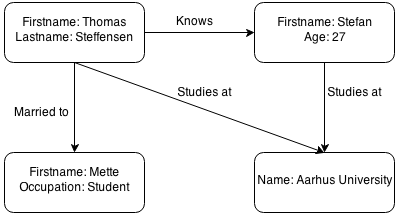
\includegraphics[scale=0.8]{Graph.png} 
	\captionsetup{format=plain,font=footnotesize,labelfont={bf,defaultCapFont},labelsep=quad,singlelinecheck=no}
	\caption[Graph store]{
		\label{fig:GraphStore}
		\footnotesize{%
			Graph store structure.
		} 
	}
\end{figure}

\section{Relational storage that scale, NewSQL}
NewSQL data stores aim to bring the relational data model into the world of horizontal scalability and flexible data models while maintaining the ACID properties and transactions of the traditional RDBMS\cite{Cattell:ScalableSQLAndNoSQLDataStores}.
NewSQL data stores does not necessarily implement a strict schema and neither do they necessarily use SQL as the query language. In fact some of them are implemented with a completely new architecture\cite{CORBETT:SpannerGooglesGloballyDistributedDatabase}.


\section{SQL, NoSQL or NewSQL?}

\section{Schema-less databases}

\section{Conclusion}